\documentclass[10pt]{book}
\usepackage{commands}


\begin{document}




\begin{tikzpicture}[remember picture,overlay]
	% If a chapter image has been specified
	\expandafter\ifstrequal\expandafter{\thechapterimage}{}{}{
		% Output the chapter image
		\node[
		anchor=north west, % Anchor point on the image
		inner sep=0pt, % Inner padding
		] at (current page.north west) {\includegraphics[angle=0,width=\paperwidth]{Images/math4OriginalSinze.jpg}};
	}
\end{tikzpicture}

\vspace{7cm}

\heading{$\mathbb{R}$eal Analysis}


%\begin{figure}[h!]
%	\centering
%	\includegraphics[width=1\linewidth]{Images/realAnalysis}
%	\caption*{$\mathbb{R}$eal Analysis, Created by DALL-E!}
%	\label{fig:realanalysis}
%	
%\end{figure}




\tableofcontents

\newpage
\chapter{Sequences and Limits}


\begin{proposition}[Sequential characterization of countable sets]
	Let $X$ be a countable set. Then, $X$ is a range of some sequence $\{x_n\}$. To put it on other words, there is an \emph{onto} function $f: \N \to X$.
\end{proposition}

\begin{problem}
	Show that the following properties hold for arbitrary countable sets.
	\begin{enumerate}[(a)]
		\item All subsets of countable sets are countable.
		\item Any union of a pair of countable sets is countable.

	\end{enumerate}
\end{problem}

\begin{proof}
	~\vspace{2pt}
	\begin{enumerate}[(a)]
		\item Let $A$ be a countable set, and $C \subseteq A$ be a subset. Since $A$ is countable, then there is a numeration for its elements, i.e.
		\[ A = \{ a_1, a_2, \cdots \}. \]
		Then for $x \in C$, there exists $n \in \N$ such that $x = a_n$. Define $g: C \to \N$, and let $g(x) = n$. Since $g$ is one-to-one, then $C$ is at most countable.
		
		\item Let $A, B$ be countable sets, and $X = A \cup B$. If $A, B$ are finite, then the statement is trivially true. But if $A, B$ are infinite, then since $A$ and $B$ are countable, then there exists bijection
		\begin{align*}
			g_A: A \to \N, \\
			g_B: B \to \N.\\
		\end{align*}
		Let $x \in A \backslash B$. Then $g_A(x) = n$ for some $n \in \N$. Define $f: X \to \N$ and let $f(x) = 2n$. Also for $y \in B$, we have $g_B(y) = m$, then define $f(y) = 2m+1$. Due to the construction, the function $f$ is one-to-one, and since $\N$ is countable, then $X$ is at most countable.

	\end{enumerate}
\end{proof}


\begin{problem}
	\label{prob:unionOfCountableManyisCountable}
	Show that the following property holds for countable sets: If
	\[ S_1, S_2, S_3, \cdots \]
	is a sequence os countable sets of real numbers,then the set $S$ formed by taking all elements that belong to at least one of the sets $S_i$ is also a countable set. 
\end{problem}

\begin{proof}
	Let
	\[ X = \bigcup_{i \in \N} S_i. \]
	Let $x \in X$. Then there exists $I \subseteq \N$ such that $\forall i \in I$ we have $x \in S_i$. Let $m = \min(I)$. Note that due to the construction of $X$, the set $I$ is not empty, and since it is a subset of natural numbers, then there exists a unique minimum. So far, we have $x \in S_m$. Since $S_m$ is countable, then there exists $f_m: S_m \to \N$ one-to-one (note that since there is a possibility that $S_m$ might be finite, then requiring $f_m$ be one-to-one, given that the co-domain is countable is enough for expressing the fact $f_m$ is at most countable). Thus $f_m(x)=n$ for some $n \in \N$. Define $F: X \to \N \times \N$, and let $F(x) = (m,n)$. Do the the construction of $F$, it is one-to-one, and since $\N \times \N$ is countable, then $X$ is at most countable. 
\end{proof}


\begin{problem}
	Let $X$ be a family of sets, and $\sim$ a relation on $X$ defined as below,
	\[ A, B \in X,\ A\sim B \biImp \exists f: A \to B,\ \text{a bijection}. \]
	In words, when $A \sim B$ we can say $A$ and $B$ have the same cardinality. Show that $\sim$ is an equivalence relation. 
	
	\textbf{A side note:} There are lots of parallel notions for this in mathematics. For example in topology, a homeomorphism (bijective and continuous) define an equivalence relation on topological spaces, in differential geometry, a diffeomorphism does the job, in group theory, an isomorphism is the parallel notion, and in general, all of these notions are generalized with the notion of morphism in category theory.
\end{problem}

\begin{proof}
	~\vspace{2pt}
	\begin{enumerate}[(a)]
		\item \textbf{Reflexivity.} Let $A \in X$. Then $id_A: A \to A$, is an bijective map (identity map). Thus $A \sim A$.
		\item \textbf{Symmetry.} Let $A, B \in X$, and $A \sim B$. Thus we know $\exists f: A \to B$, a bijection. Let $g = f^{-1}: B \to  A$. Due to the construction $g$ is also bijective. Thus $B \sim A$.
		\item \textbf{Transitivity.} Let $A, B, C \in X$, $A \sim B$, and $B \sim A$. Then $\exists f: A\to B$ and $g: B \to C$ injective. Define $h: A \to B$, $h = g \circ f$. Due to the construction, $h$ is also bijective. Thus $A \sim C$.
	\end{enumerate}
\end{proof}


\begin{problem}
	We define a real number to be \emph{algebraic} is it is a solution of some polynomial equation
	\[ a_n x^n + a_{n-1}x^{n-1} + \cdots + a_1 x + a_0 = 0, \]
	where all the coefficients are integers. A real number that is not algebraic, is called a transcendental number. Prove that the set of all algebraic numbers is countable.
\end{problem}

\begin{proof}
	The set of all polynomials of degree $n-1$ is identified with $\Z^{n}$, which is countable. Thus the set all such polynomials is 
	\[  X = \bigcup_{n\in\N} \Z^{n}.\]
	As we proved in the Problem \autoref{prob:unionOfCountableManyisCountable}, $X$ is countable. On the other hand, every polynomial has a countable number of zeros. Thus The set of all zeros of all polynomial with integer coefficients is countable.
\end{proof}

\begin{problem}
	Let $\seq{s}$ be a sequence in $\R$ converging to $L \in \R$. Prove that the following definition is the equivalent to the original definition of converges.
	\[ \forall m \in \N,\ \exists N\in\N:\ \forall n> N \wh \abs{s_n - L} < 1/m.  \]
	\textbf{Side note.} This is a useful equivalent definition of convergence, because to check a sequence converges is enough to check the definition above for the integer $m$'s only.
\end{problem}
\begin{proof}
	The fact that the original definition implies the definition above is trivial. It suffice to let $\epsilon = 1/m$. However, for the converse, we assume that the definition above is true and we want to infer the original definition of convergence. Let $\epsilon>0$ is give. Then $\exists m \in \N$ such that $1/m < \epsilon$ (The Archimedes property for real numbers). On the other hand since we have assumed that the altered definition is true, them $\exists N \in \N$ such that $\forall n >N$ we have
	\[ \abs{s_n - L} < 1/m < \epsilon. \]
	This completes the proof.
\end{proof}


\begin{problem}
	If $\{s_n\}$ is a sequence of positive real numbers converging to a positive number $L$, show that $\{\sqrt{s_n}\}$ converges to $\sqrt{L}$.
\end{problem}
\begin{proof}
	Since $s_n \to L$, then $\exists N_1 > 0$ such that $\forall n > N_1$ we have $s_n < L+1$. Thus $\sqrt{s_n}<\sqrt{L+1}$, which implies $\sqrt{s_n} + \sqrt{L} < \sqrt{L+1} + \sqrt{L} = M$, for $M \in \R$. For a given $\epsilon>0$ let $\epsilon_0 = M \epsilon$. We know $\exists N_2>0$ such that $n>N_2$ we have $\abs{s_n - L} = \abs{\sqrt{s_n} - \sqrt{L}} \abs{\sqrt{s_n}+\sqrt{L}} < \epsilon_0$. Then $\abs{\sqrt{s_n} - \sqrt{L}} < \epsilon_0 /M = \epsilon $. This completes the proof.
\end{proof}


\begin{problem}
	Show that the sequence 
	\[ a_n = n^p + \alpha_1 n^{p-1} + \alpha_2 n^{p-2} + \cdots + \alpha_p  \]
	diverges to $\infty$, where $p$ is a positive integer and $\alpha_1, \alpha_2, \cdots, \alpha_p$ are real numbers (positive or negative). 
\end{problem}

\begin{proof}
	We construct the sequence $\{b_n\}$ such that $b_n \leq a_n$ always hold.
	\[ b_n = n^p - \abs{\alpha_1}n^{p-1} -\abs{\alpha_2}n^{p-2}  - \cdots - \abs{\alpha_p}. \]
	To demonstrate the proof in a more clear way, we assume $p=4$. Now we can solve the following inequalities
	\begin{align*}
		1/4 n^4 - \abs{\alpha_1}n^3 > 1/8 n^4 &\implies n > \abs{8\alpha_1},\\
		1/4 n^4 - \abs{\alpha_2}n^2 > 1/8 n^4 &\implies n > \abs{8\alpha_2}^{1/2},\\
		1/4 n^4 - \abs{\alpha_3}n^1 > 1/8 n^4 &\implies n > \abs{8\alpha_3}^{1/3},\\
		1/4 n^4 - \abs{\alpha_4}n > 1/8 n^4 &\implies n > \abs{8\alpha_4}^{1/4},\\
	\end{align*}
	Let $N = \max\{ \abs{8\alpha_1}, \abs{8\alpha_2}^{1/2},\abs{8\alpha_3}^{1/3},\abs{8\alpha_4}^{1/4}\}$. Then for $n > N$ all of the inequalities above holds. Thus we can write
	\[  n^4 + \alpha_1 n^3 + \alpha_2 n^2 + \alpha_3 n + \alpha_4 > n^4 - \abs{\alpha_1}n^3 - \abs{\alpha_2}n^2 - \abs{\alpha_3} n - \abs{\alpha_4} > 1/2 n^4. \]
	Since the very last term ($1/2n^4$) diverges, then the sequence $a_n$ diverges.
\end{proof}


\begin{problem}
	Prove that if $\seq{s}$ bounded, then $\{s_n/n\}$ converges.
\end{problem}
\begin{proof}
	We propose that the $s_n/n \to 0$. Since $s_n$ is bounded, then there is $M>0$ such that $\abs{s_n}<M$ for all $n \in \N$. For a given $\epsilon>0$, let choose a natural number $N>M/\epsilon$. Then $\forall n>N$ we have
	\[ \abs{s_n/n} < \abs{s_n}/\abs{n} < M/\abs{n} < M\epsilon/M = \epsilon. \]
	This implies that $\{s_n/n\}$ converges to zero.
\end{proof}

\begin{problem}[Order property in limits]
	Let $\seq{t}$ and $\seq{s}$ be two real sequences that converge to $T$ and $S$ respectively, and also $\forall n \in \N$ we have $s_n \leq t_n$. Prove that $T \leq S$
	
	\textbf{Side note:} By this proof you will show that the limits preserve the order property, and this fact is the main idea behind the squeeze theorem.
\end{problem} 

\begin{proof}
	Since $t_n \geq s_n$ for all $n\in\N$, then $t_n - s_n \geq 0$. Thus $t_n - s_n \pm T \pm S < 0$, and we can re-arrange the terms as $(t_n - T) + (S - s_n) + (T-S) >0$. On the other hand, since $s_n \to S$ and $t_n \to T$, then for $\epsilon>0$ there exists $N_1 > 0, N_2 > 0$ such that $n>N_1$ implies $\abs{s_n - S} < \epsilon/2$ and $n>N_2$ implies $\abs{t_n - T} < \epsilon/2$. Let $N = \max\{N_1,N_2\}$. So $\forall n>N$ we will have
	\[ \epsilon/2 + \epsilon/2 + (T-S) > (t_n - T) + (S - s_n) + (T-S) > 0. \]
	This implies $T-S > -\epsilon$ for all $\epsilon>0$. Thus we conclude $T- S \geq 0 \implies T > S$.
\end{proof}


\begin{problem}
	A careless student gives the following as a proof of the squeeze theorem. Find the flaw:
	
	"If \(\lim_{{n \to \infty}} s_n = \lim_{{n \to \infty}} t_n = L\), then take limits in the inequality \(s_n \leq x_n \leq t_n\) to get \(L \leq \lim_{{n \to \infty}} x_n \leq L\). This can only be true if \(\lim_{{n \to \infty}} x_n = L\)."
	
\end{problem}
\begin{proof}
	Formally, the student turns the inequality into two pieces, i.e. $s_n \leq x_n$ and $x_n \leq t_n$ and tries to apply the order property of limits to each of them. But the problem is that the squeeze theorem only states that $s_n$ and $t_n$ has limits and does not have any information about the existence of limit for $x_n$. Thus we can not simply apply the limit to the inequality and infer the squeeze theorem.
\end{proof}

\begin{problem}
	Let $\{s_n\}$ be a sequence of positive numbers. Show that the condition
	\[ \lim_{n\to\infty} \frac{s_{n+1}}{s_n} < 1 \]
	implies $s_n \to 0$.
\end{problem}
\begin{proof}
	Let $\lim_{n\to\infty}\frac{s_{n+1}}{s_n} = \alpha < 1 $. Also, since $\forall n\in\N$ we have $s_n > 0$, then $\alpha\geq0$. So $0 \leq \alpha < 1$. Define $d = (1-\alpha)/2$, thus $1/2 \leq d < 1$ and $d > \alpha$ (in fact, $d$ is sandwiched between $\alpha$ and 1). Since $s_{n+1}/s_n \to \alpha$, then $\exists N_1 > 0$ such that $\forall n>N_1$ we have
	\[ \frac{s_{n+1}}{s_n} < d \implies s_{n+1}<d s_n \implies s_{n+1}< d s_n < d^2 s_{n-1} < \cdots < d^n s_1. \]
	Since all $s_n$ are positive, then $s_1 = c d$, for some $c \in \R$. Thus we can write the inequality above as
	\[ s_{n+1} < d^{n+1}c \implies s_n < d^n c. \]
	Now we can proceed with the $\epsilon-N$ proof directly, or we can use squeeze theorem. We know that 
	\[ 0 \leq s_n < d^n c. \]
	Since both $0$ and $d^n$ converges to zero, then $s_n$ also converges to zero, i.e. $s_n \to 0$.
\end{proof}

\begin{problem}
	Let $\{s_n\}$ be a sequence of positive numbers. Show that the condition
	\[ \lim_{n\to\infty} \frac{s_{n+1}}{s_n} > 1 \]
	then $s_n \to \infty$.
\end{problem}

\begin{proof}
	Let $\lim_{n\to\infty} \frac{s_{n+1}}{s_n} = \alpha > 1$. Define $d = 1 + (\alpha - 1)/2$ (in fact $d$ is sandwiched between 1 and $\alpha$). Since $s_{n+1}/s_n \to \alpha$, then $\exists N>0$ such that $\forall n>N$ we have $s_{n+1}/s_n > d$. As we seen in the solution of the problem above, this implies 
	\[ s_n > d^n c, \]
	where $c = s_1/d$. Now we can proceed with the $M-N$ proof to show that $s_n$ actually diverges.
\end{proof}

\begin{problem}
	Let $\{s_n\}$ be a real sequence that is non-decreasing and bounded. Then prove that 
	\[ s_n \to \sup_{n\in\N}(s_n). \]
\end{problem}
\begin{proof}
	Let $L = \sup_{n\to \infty} s_n$. Since $s_n \in \R$ for all $n \in \N$, and is bounded, then the suprimum exists and $L \in \R$. Let $\epsilon>0$ be given, and define $\beta = L - \epsilon$. Since $L$ is the least upper bound for the sequence, then for $\exists N \in \N$ such that $s_N > \beta$, and since $s_n$ is non-decreasing, $\forall n>N$ we have $s_n > \beta \implies \abs{s_n - L} < \epsilon$. This implies that $s_n \to L$ as $n\to\infty$.
\end{proof}

\begin{problem}
	Decide on the convergence of the following sequence.
	\[ \sqrt{2}, \sqrt{2+\sqrt{2}}, \sqrt{2+\sqrt{2+\sqrt{2}}}, \cdots \]
\end{problem}

\begin{proof}
	This sequence converges, since it is increasing and bounded. The fact that this sequence is increasing is trivial, but for being bounded we start with
	\[ \boxed{\sqrt{2}< 2}  \implies 2+\sqrt{2} < 4 \implies \boxed{\sqrt{2+\sqrt{2}} < 2} \implies 2+\sqrt{2+\sqrt{2}}<4 \implies \boxed{\sqrt{2+\sqrt{2+\sqrt{2}}<2}} \implies \cdots. \]
	Thus as we can see, all of the terms of the sequence is less than 2. Thus this sequence converges.
\end{proof}
\afterpage{\null\newpage}

\chapter{Sets and Mappings}

\begin{remark}
	Let $\R_+$ denote the real number greater than or equal to zero\footnote{This note is from Segel, undergraduate analysis.}. The we can view the association $x \mapsto x^2$ as a map from $R$ to $\R_+$. When viewed so, the map is the surjective. Thus it is a reasonable convention not to identify this map with the map $f:\R \to \R$ defined by the same formula. To be completely accurate, we should therefore denote the set of arrival and the set of departure of the map into our notation, and for instance write
	\[ F^S_T: S \to T, \]
	instead of our $f: S \to T$ notation. In practice, this notation is too clumsy, so that we omit the indices $S, T.$ However, the reader should keep in mind the distinction between the maps 
	\[ f^\R_{\R_+}: \R \to \R_+ \quad \text{and} \quad f_\R^\R: \R \to \R  \]
	both defined by the association $x \mapsto x^2$. The first map is surjective, while the second one is not. Similarly the maps
	\[ f_{\R_+}^{R_+}: \R_+ \to \R_+ \quad \text{and} \quad f_\R^{\R_+}: \R_+ \to \R \]
	defined by the same association $x \mapsto x^2$ are injective.
\end{remark}

\begin{remark}

\end{remark}
\newpage
\section{Basics}
Partial differential equations relate the partial derivatives of a function to each other. For example $f$ can be a function of spacial coordinates (like $x,y,z$ in the case of Cartesian coordinates), dynamical variable (like time), or any other kind of variables (like the space of genotypes g). For example suppose that $ \Phi(x,y) $ represents the electric potential of a point charge. Such function should satisfy the Laplace equation:

\[	 \partial_{xx} \Phi + \partial_{yy} \Phi = 0.	\]
Note that the symbols $ \partial_{xx} $ and $ \partial_{yy} $ are short symbols for $ \frac{\partial^2}{\partial x^2} $ and $ \frac{\partial^2}{\partial y^2} $ respectively.

\begin{defbox}{Order of PDE}
	The order of a PDE is the highest derivative that occurs in the equation. 
\end{defbox}

Based on the definition above, the Laplace equation is a second order partial differential equation. 

\subsection{Classification of The Second Order PDEs }

There are three categories of the second order PDEs that every other type of a second order PDE can be converted to one of these kinds. The most general type of a second order PDE can be written as:

\begin{equation}
	A \partial_{xx} u + B \partial_{xy} u + C \partial_{yy} u + D \partial_{x} u + E \partial_{y} u + F u = k
	\label{equ:GeneralSecondOrderPDE}
\end{equation}

In which the coefficients are all a function of $x,y$ (but not $ u $ in which case the PDE will be nonlinearx). Equation \ref{equ:GeneralSecondOrderPDE} can be summarized in a more compact form using the derivative operator $ \operatorname{L} $: 

\[	 \operatorname{L} u = 0,	\]

in which:

\[  \operatorname{L} = A \partial_{xx} + B \partial_{xy} + C \partial_{yy} + D \partial_{x} + E \partial_{y} + F \].

Because of the similarities of the equation \ref{equ:GeneralSecondOrderPDE} with the generic quadratic equation describing the conic sections, we call each class of second order PDEs with its corresponding conic section. The generic equation describing the conic sections is:

\begin{equation}
	A x^2 + B x y + C y^2 + D x + E y + K = 0.
	\label{equ:ConicSections}
\end{equation}


All of the conic sections (ellipse, parabola, hyperbola) can be described with the equation \ref{equ:ConicSections} which is determined with the discriminant $ \Delta = B^2 - 4 A C $. for $ \Delta=0 $, $ \Delta > 0 $, and $ \Delta < 0 $ the conic section will be \textbf{parabolic}, \textbf{hyperbolic}, and \textbf{elliptic} respectively. Table \ref{tab:PDE-types} summarizes special categories of the linear second order PDEs that frequently occur in physical applications. \newline


\begin{table}[]
	\centering
	\resizebox{\textwidth}{!}{%
		\begin{tabular}{|c|c|c|c|c|}
			\hline
			PDE                     & Analogous conic sec. & $\Delta$     & Class      & Application               \\ \hline
			$ u_t = u_{xx}$         & $T = x^2$           & 0            & parabolioc & Diffusion - Heat Equation \\ \hline
			$ u_{tt} = u_{xx} $     & $T^2 = x^2$         & $\Delta > 0$ & Hyperbolic & Wave Equation             \\ \hline
			$ u_{xx} + u_{yy} = 0 $ & $x^2 + y^2 = 0$ & \multirow{2}{*}{$\Delta < 0$} & \multirow{2}{*}{Elliptic} & Laplace \\ \cline{1-2} \cline{5-5} 
			$ u_{xx} + u_{yy} = c $ & $x^2 + y^2 = k$     &              &            & Poisson                   \\ \hline
		\end{tabular}%
	}
	\caption{A summary of the three class of second order linear PDE.}
	\label{tab:PDE-types}
\end{table}


\subsection{Intuitive Derivation of the Second Order PDEs}
The three classes of the second order linear PDEs in table \ref{tab:PDE-types} can be derived intuitively using the continuity law (conservation law) and the constitutive law that is determined by the nature of the problem which is the subject of the following sections. 
 
\subsubsection{Continuity Equation or Conservation Laws}
The most important part of deriving the PDE equations is the continuity law or conservation law. This fact is imposed because of our common sense about nature. Suppose that we want to study the concentration of of a red ink in a infinitesimal cube. The continuity equation, in simple terms, state that the change of the concentration of the ink inside the infinitesimal cube is equal to the ink that has entered the cube from outside from its boundaries (we are assuming no source or sink of ink inside the cube). For instance, consider the infinitesimal box in figure \ref{fig:infbox}. The change of the concentration of the ink inside the cube is $\frac{\partial c}{\partial t}$. Because we know that there are no sources or sinks of ink inside the cube, then the change in the concentration is equal to the amount that comes in and goes out from the boundaries of the box. To put this in numbers, we introduce the important vector quantity \emph{flux} $ \Phi $. Flux is the amount of particles flow per unit area per unit time (see figure \ref{fig_fluxCrossSection}).


\begin{figure}[h!]
	\centering
	\tikzset{every picture/.style={line width=0.75pt}} %set default line width to 0.75pt        
	
	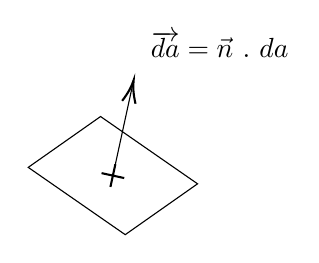
\begin{tikzpicture}[x=0.75pt,y=0.75pt,yscale=-1,xscale=1]
		%uncomment if require: \path (0,300); %set diagram left start at 0, and has height of 300
		
		%Flowchart: Data [id:dp7886171984971329] 
		\draw   (233.06,82.54) -- (279.79,114.96) -- (244.94,139.46) -- (198.21,107.04) -- cycle ;
		%Straight Lines [id:da19634912279776984] 
		\draw    (239,111) -- (248.58,66.95) ;
		\draw [shift={(249,65)}, rotate = 102.26] [color={rgb, 255:red, 0; green, 0; blue, 0 }  ][line width=0.75]    (10.93,-3.29) .. controls (6.95,-1.4) and (3.31,-0.3) .. (0,0) .. controls (3.31,0.3) and (6.95,1.4) .. (10.93,3.29)   ;
		\draw [shift={(239,111)}, rotate = 282.26] [color={rgb, 255:red, 0; green, 0; blue, 0 }  ][line width=0.75]    (-5.59,0) -- (5.59,0)(0,5.59) -- (0,-5.59)   ;
		
		% Text Node
		\draw (256,40) node [anchor=north west][inner sep=0.75pt]   [align=left] {$\displaystyle \overrightarrow{da} =\vec{n} \ .\ da$};
	\end{tikzpicture}
	\caption{The dot product $\protect\overrightarrow{\Phi}.\protect\overrightarrow{da}$ is the amount of particles passing through the infinitesimal cross section in unit time.}
	\label{fig_fluxCrossSection}
\end{figure}


\begin{figure}[h!]
	\centering
	\tikzset{every picture/.style={line width=0.75pt}} %set default line width to 0.75pt        
	
	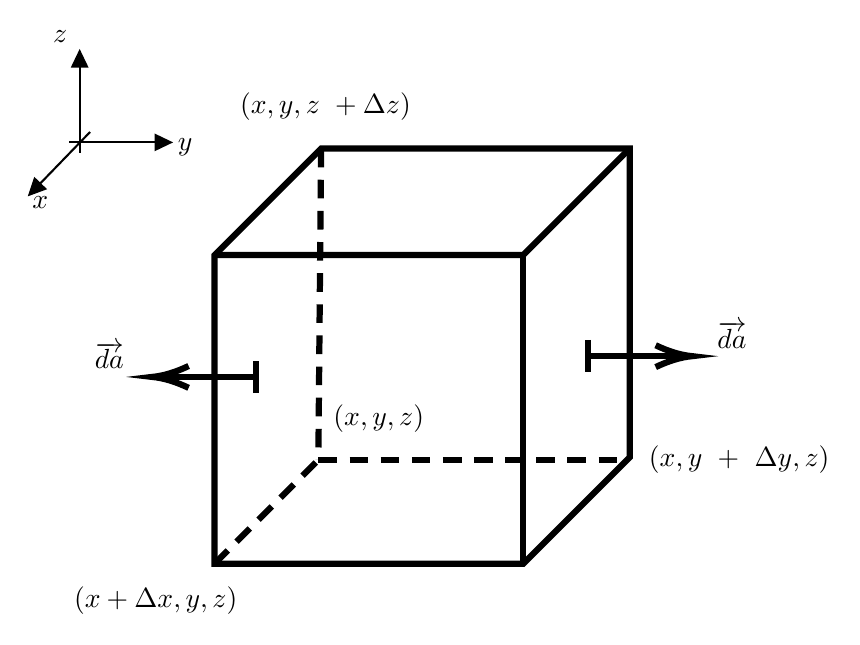
\begin{tikzpicture}[x=0.75pt,y=0.75pt,yscale=-1,xscale=1]
		%uncomment if require: \path (0,300); %set diagram left start at 0, and has height of 300
		
		%Shape: Cube [id:dp6052690098400888] 
		\draw  [line width=2.25]  (200,101.31) -- (251.31,50) -- (400,50) -- (400,198.69) -- (348.69,250) -- (200,250) -- cycle ; \draw  [line width=2.25]  (400,50) -- (348.69,101.31) -- (200,101.31) ; \draw  [line width=2.25]  (348.69,101.31) -- (348.69,250) ;
		%Straight Lines [id:da6838346844891714] 
		\draw [line width=2.25]  [dash pattern={on 6.75pt off 4.5pt}]  (250,200) -- (400,200) ;
		%Straight Lines [id:da4358863669422177] 
		\draw [line width=2.25]  [dash pattern={on 6.75pt off 4.5pt}]  (251.31,50) -- (250,200) ;
		%Straight Lines [id:da8699451449684632] 
		\draw [line width=2.25]  [dash pattern={on 6.75pt off 4.5pt}]  (200,250) -- (250,200) ;
		%Straight Lines [id:da6153923820857115] 
		\draw [line width=2.25]    (220,160) -- (174,160) ;
		\draw [shift={(170,160)}, rotate = 360] [color={rgb, 255:red, 0; green, 0; blue, 0 }  ][line width=2.25]    (17.49,-5.26) .. controls (11.12,-2.23) and (5.29,-0.48) .. (0,0) .. controls (5.29,0.48) and (11.12,2.23) .. (17.49,5.26)   ;
		\draw [shift={(220,160)}, rotate = 360] [color={rgb, 255:red, 0; green, 0; blue, 0 }  ][line width=2.25]    (0,7.83) -- (0,-7.83)   ;
		%Straight Lines [id:da3502060568264709] 
		\draw [line width=2.25]    (380,150) -- (426,150) ;
		\draw [shift={(430,150)}, rotate = 180] [color={rgb, 255:red, 0; green, 0; blue, 0 }  ][line width=2.25]    (17.49,-5.26) .. controls (11.12,-2.23) and (5.29,-0.48) .. (0,0) .. controls (5.29,0.48) and (11.12,2.23) .. (17.49,5.26)   ;
		\draw [shift={(380,150)}, rotate = 180] [color={rgb, 255:red, 0; green, 0; blue, 0 }  ][line width=2.25]    (0,7.83) -- (0,-7.83)   ;
		%Straight Lines [id:da8422422028495438] 
		\draw [line width=0.75]    (140,42) -- (112.09,70.84) ;
		\draw [shift={(110,73)}, rotate = 314.06] [fill={rgb, 255:red, 0; green, 0; blue, 0 }  ][line width=0.08]  [draw opacity=0] (8.93,-4.29) -- (0,0) -- (8.93,4.29) -- cycle    ;
		%Straight Lines [id:da7449366310627421] 
		\draw [line width=0.75]    (135,52) -- (135,5) ;
		\draw [shift={(135,2)}, rotate = 90] [fill={rgb, 255:red, 0; green, 0; blue, 0 }  ][line width=0.08]  [draw opacity=0] (8.93,-4.29) -- (0,0) -- (8.93,4.29) -- cycle    ;
		%Straight Lines [id:da9487980467676893] 
		\draw [line width=0.75]    (130,47) -- (177,47) ;
		\draw [shift={(180,47)}, rotate = 180] [fill={rgb, 255:red, 0; green, 0; blue, 0 }  ][line width=0.08]  [draw opacity=0] (8.93,-4.29) -- (0,0) -- (8.93,4.29) -- cycle    ;
		
		% Text Node
		\draw (256,172) node [anchor=north west][inner sep=0.75pt]   [align=left] {$\displaystyle ( x,y,z)$};
		% Text Node
		\draw (131,260) node [anchor=north west][inner sep=0.75pt]   [align=left] {$\displaystyle ( x+\Delta x,y,z)$};
		% Text Node
		\draw (408,192) node [anchor=north west][inner sep=0.75pt]   [align=left] {$\displaystyle ( x,y\ +\ \Delta y,z)$};
		% Text Node
		\draw (211,22) node [anchor=north west][inner sep=0.75pt]   [align=left] {$\displaystyle ( x,y,z\ +\Delta z)$};
		% Text Node
		\draw (111,72) node [anchor=north west][inner sep=0.75pt]   [align=left] {$\displaystyle x$};
		% Text Node
		\draw (181,44) node [anchor=north west][inner sep=0.75pt]   [align=left] {$\displaystyle y$};
		% Text Node
		\draw (121,-8) node [anchor=north west][inner sep=0.75pt]   [align=left] {$\displaystyle z$};
		% Text Node
		\draw (141,142) node [anchor=north west][inner sep=0.75pt]   [align=left] {$\displaystyle \overrightarrow{da}$};
		% Text Node
		\draw (441,132) node [anchor=north west][inner sep=0.75pt]   [align=left] {$\displaystyle \overrightarrow{da}$};
		
		
	\end{tikzpicture}
	\caption{The infinitesimal cube for deriving the continuity equation}
	\label{fig:infbox}
\end{figure}



\newpage

Let's get back to the infinitesimal cube in figure \ref{fig:infbox} and derive the continuity equation. We can start we tracking the net change in the number of particles inside the cube due to the flux in x direction:

\begin{align*}
	-\frac{dN_x}{dt} &= \Phi_x(x,y,z) . (-dz dy) + \Phi_x(x +dx, y,z) . (dzdy) \\
	 				&= (\Phi_x(x+dx,y,z)-\Phi_x(x,y,z))dydz 
\end{align*}

Note that the negative sign in the LHS of the equation above is simply to match the meaning of the two sides of the equations. For instance, if the RHS of the equation above is positive, it means that the net change of the number of particles in the box in negative (meaning that particles are leaving the box) which is equivalent to $ -\frac{dN}{dt} $. Similarly in the y and z direction:

\begin{align*}
	-\frac{dN_y}{dt} &= (\Phi_y(x,y+dy,z)-\Phi_y(x,y,z)) dx dz \\
	-\frac{dN_z}{dt} &= (\Phi_z(x,y,z+dz) - \Phi_z(x,y,z)) dx dy
\end{align*}

So the net change in the number of particle in the box per $dt$ will be:

\begin{align*}
	-\frac{dN}{dt} &= - (\frac{dN_x}{dt} + \frac{dN_y}{dt} + \frac{dN_z}{dt}) \\
	&= (\Phi_x(x+dx,y,z)-\Phi_x(x,y,z))dydz + \\
	&\, (\Phi_y(x,y+dy,z)-\Phi_y(x,y,z)) dx dz + \\
	&\, (\Phi_z(x,y,z+dz) - \Phi_z(x,y,z)) dx dy
\end{align*}


By dividing the both sides of the above equation by the volume of the cube $ dV = dx dy dz $ we can write:

\begin{equation*}
	\frac{dc}{dt} = - (\partial_{x}\Phi_x + \partial_{y}\Phi_y + \partial_{z}\Phi_z) = -\mathbf{\nabla} . \Phi
\end{equation*}

In which $c = N/V$ is the concentration, $ \nabla $ is the divergence operator, and $ \Phi $ is the flux. 

\begin{defbox}{Continuity Equation}
	The following important relation is known as the continuity equation(or conservation law):
	
	\begin{equation}
			\frac{dc}{dt} + \mathbf{\nabla} . \Phi = 0
	\end{equation}

	in which $\Phi$ is the flux, $c$ is the concentration, and $ \nabla $ is the divergence operator.
\end{defbox}


\subsubsection{Conservation Law for Momentum}
will be used to derive the wave equation


\subsection{Constitutive Laws: Advection, Diffusion and Wave Equation}

Having the continuity equation in hand makes the derivation PDEs very straight forward. We only need to insert the constitutive laws (which are enforced by the nature of the problem) in the continuity equations derived in the section above.


\begin{itemize}
	\item Fick's Law $\rightarrow$ Constitutive law for diffusion 
	\item Hook's law $\rightarrow$ Constitutive law for the wave equation
\end{itemize}




\newpage
\chapter{Hausdorff Topological Spaces}



The following is a section of the great book ``Mathematical Discovery'' by Bruckner.
\begin{quote}
	Professional mathematicians must adhere to strict standards in their work. This entails providing precise definitions, even for seemingly familiar concepts. Such precision often requires the use of complex technical tools and methods. A mathematician must possess a clear understanding of fundamental concepts, such as the precise definition of a "curve," the mathematical interpretation of "traversing a curve with the inside to the left," the formal description of the number of "holes" in a pretzel, and the mathematical definition of area.
	
	\textbf{	It's important to note that this level of rigor and precision is not typically present when a mathematician initially approaches a problem and begins working on a solution.} In the early stages, ideas tend to be more abstract and intuitive. The refinement and meticulousness become evident only in the final drafts of mathematical work.
\end{quote}

Thus, we first need to have a discussion that show that the ideas behind the abstractions and generalizations are achievable by careful studying the mathematical objects already around us. This this section focuses to motivate the reader towards the more abstract concepts.

Thus we will discuss that the $\R^n$ along with the Euclidean distance has some special properties (which later will be generalized to the concept of metric spaces), and then we will see that the notion of Euclidean distance give rise to special sets called open ball which will give rise to the notion of open sets. We will study the properties of these open sets and later we will study what if we define the notion of open sets on its own (without any need to any particular metric) which will lead to the notions and ides of topological spaces. 

\section{Motivation}
Consider the set $\R^k$ which is a $k$ fold Cartesian product of our favorite set $\R$!. We can also extend the notion of Euclidean distance in $\R$ (which was simply $\abs{x-y}$ for $x,y\in\R$) to $\R^k$ as follows
\[ \abs{x-y} = \sqrt{\sum_{i=1}^{k} (y_i - x_i)^2}, \qquad x=(x_1,\cdots,x_k),\ y=(y_1,\cdots,y_k) \in \R^k. \]

We can easily observe that the Euclidean distance is a function $d:\R^k\times \R^k \to\R$ that satisfies the following properties
\begin{enumerate}[(i)]
	\item $\abs{x-y} \geq 0, \quad \abs{x-y}=0 \biImp x=y$,
	\item $\abs{x-y} = \abs{y-x}$,
	\item $\abs{x-y} \leq \abs{x-z} + \abs{z-y}$
\end{enumerate}
Later, We will study the generalized idea of such functions defined on a set which will give rise to the concept of metric spaces.

Now, we intuitively define the notion of ``open ball'' centered at $x\in\R^k$ with radius $r\in\R$ as follows
\[ \ball{x}{r} = \{ y\in\R^k:\ \abs{x-y}<r \}. \]
Then we define a set $A\subseteq\R^k$ to be a open set such that for every element $x\in\A$, we can have an open ball $\ball{x}{r}$ for some $r\in\R$ which is contained in $A$. More formally we can write
\[ \forall x \in A,\ \exists r>0 \st x\in\ball{x}{r}\subseteq\R^k. \] 
Since this notion is a very central one (as we will find out later), for $\R^k$, we have the notion of the set of all open sets of $\R^k$, for which we write $\mathcal{T}$.
 
Then we can go a little bit beyond the immediate intuition and define the notion of the set of all neighborhoods of $x$ as
\[ \mathcal{N}(x) = \{ S\subseteq \R^k:\ \exists u\in\mathcal{T},\ x\in u\subseteq S \} . \]
It immediately follows from the definition that all open balls containing $x$ (not necessarily containing $x$) are in $\mathcal{N}(x)$, along with other sets which satisfies the required property. We are now in a good shape to study the properties of the open sets $u\in\mathcal{T}$. We claim the followings are some of such properties (which as it will turn out are the central properties in some sense)
\begin{enumerate}[(i)]
	\item \[\emptyset,\ \R^k \in \mathcal{T}.\]
	\item \[\forall \mathcal{G} \subseteq \mathcal{T} \wh \bigcup_{g\in\mathcal{G}}g \in \mathcal{T}.\]
	\item \[ U_1,\cdots,U_n \in \mathcal{T},\ n\in\N \implies \bigcap_{i=1}^{n}U_i \in \mathcal{T}.\]
	\item \[ \forall x,y\in\R^k,\ \exists U,V \in \mathcal{T} \st x\in U,\ y\in V,\quad U\cap V = \emptyset. \]
\end{enumerate}


\begin{proof}
	TO BE ADDED.
\end{proof}

Since the notion of open sets is closely related with the distance function, thus there is no surprise that it can be used to express the ideas of convergence of a sequence in $\R^k$ (such a fundamental concept in analysis) with the new terminology. For instance, the following two statements are logically equivalent for $x_n\to\hat{x}$
\begin{enumerate}[(i)]
	\item $\forall \epsilon>0,\ \exists N>0,\st \forall n>N \wh \abs{x_n-\hat{x}} < \epsilon$.
	\item $\forall S \in \mathcal{N}(\hat{x}),\ \exists N>0,\st \forall n > N \wh x_n \in S$.
\end{enumerate}
\begin{proof}
	TO BE ADDED.
\end{proof}

\section{Metric Spaces}
Although $\R^k$ is a very useful set synthesized in a special way to meet most of our requirements (for instance the completeness arguments in the sense of Cauchy sequence, least upper bound property, and etc.) but not every set we encounter is $\R^k$. We can have sets that are globally very different than the ``\emph{flat}'' $\R^k$, for instance $\mathbb{S}^1$ (unit circle), $\mathbb{S}^1 \times \mathbb{S}^1$ (a tours), etc. One of the main approaches in dealing with such structures is to ``locally'' convert it  (in a useful way) to a collection (or atlas) of subsets of $\R^k$ and then work with the original ``alien'' set in an indirect way by focusing on these local images in $\R^k$. Apart from this approach, it is also useful to generalize the notions of distance in a set, which will enable us working with other classes of abstract structures without relying on $\R^k$, as some of them are way larger than $\R^k$. For instance, consider the set of all bounded function $f:[0,1]\to\R$. This set has a cardinality that is bigger than the cardinality of continuum. Also, might want to work with sets that are discrete in nature, like $\N$ which their cardinality is less than $\R^k$. So relying on $\R^k$ for all purposes is not feasible, thus it might be a good idea to have the notion of distance between elements in set.

\begin{defbox}[Metric Space]
	A metric space is simply $(X,d)$ in which $X$ is a  set and $d:X\times X \to \R$ is a function called metric that satisfies the following properties
	
	\begin{enumerate}[(i)]
		\item $d(x,y) \geq 0,\quad d(x,y) =0 \biImp x=y$.
		\item $d(x,y) = d(y,x)$.
		\item $d(x,y) \leq d(x,z) + d(z,y)$.
	\end{enumerate}
	In which $x,y,z\in X$. 
\end{defbox}
Now we can easily see that all of the notions like open balls, open sets, and etc. which we defined for $\R^k$ can also be defined for a metric space. We can define different metrics on a particular set based on our demands. In fact there are infinitely many ways to come up with a metric function. \textbf{One of our main tasks in studying metric spaces is to show that there are some properties of a metric space that are independent of a particular defined metric}. As we will see later, this will give rise to more abstract construct called topological spaces. 

\begin{defbox}[Open Ball in $\R^k$]
	Let $(X,d)$ be a metric space. An open ball centered at $x\in X$ with radius $r$ is the set
	\[ \ball{r}{x} = \{ y\in X: d(y,x)<r \}, \]
\end{defbox}


\begin{defbox}[Open Set in $\R^k$]
	Let $(X,d)$ be a metric space and let $U\subseteq X$. $U$ is open if 
	\[ \forall x\in X,\ \exists \ball{r}{x} \st \ball{r}{x} \subseteq U. \]
	We denote the set of all open sets of $X$ as $\mathcal{T}$.
\end{defbox}

A very useful intuition about open sets is that we can move around any points of the set (sufficiently small) and still be in the set. In other words, we can perturb the points of an open set (a sufficiently small perturbation) and still remain in the set. 

\begin{defbox}[Neighborhood of $x$]
	Let $(X,d)$ be a metric space. Then the set of all neighborhoods of $x$ is
	\[ \mathcal{N}(x) = \{ S \in \mathcal{P}(X):\ \exists U \in \mathcal{T} \st x\in U \subseteq S\}. \]
	In other words, A neighborhood of $x\in X$, is the collection of all subsets of $X$, such that contains an open set containing $x$.
\end{defbox}

\begin{remark}
	An open ball is an open set. This is not a tautological statement. The word ``open'' in the notion of open ball, has nothing to do with the word ``open'' in the notion of open set. however, we can show that an open ball is indeed an open set, thus deserves the name ``open''. In more accurate language 
	\begin{quote}
		Let $\hat{x}\in X,\ \hat{r}\in\R,\ \text{and define } U=\ball{\hat{r}}{\hat{x}}$. Then $U$ is an open set.
	\end{quote}
\end{remark}
\begin{proof}
	The proof of remark above can be facilitated by considering the following diagram.

	\begin{figure}[h!]
	\centering
	
	
	
	
	
	\tikzset{every picture/.style={line width=0.75pt}} %set default line width to 0.75pt        
	
	\begin{tikzpicture}[x=0.75pt,y=0.75pt,yscale=-1,xscale=1]
		%uncomment if require: \path (0,300); %set diagram left start at 0, and has height of 300
		
		%Shape: Arc [id:dp8474273111700028] 
		\draw  [draw opacity=0][dash pattern={on 4.5pt off 4.5pt}] (237.52,62.7) .. controls (251.49,54.62) and (267.7,50) .. (285,50) .. controls (337.47,50) and (380,92.53) .. (380,145) .. controls (380,161.12) and (375.99,176.3) .. (368.9,189.59) -- (285,145) -- cycle ; \draw  [dash pattern={on 4.5pt off 4.5pt}] (237.52,62.7) .. controls (251.49,54.62) and (267.7,50) .. (285,50) .. controls (337.47,50) and (380,92.53) .. (380,145) .. controls (380,161.12) and (375.99,176.3) .. (368.9,189.59) ;  
		%Shape: Circle [id:dp7267488539784774] 
		\draw  [fill={rgb, 255:red, 65; green, 117; blue, 5 }  ,fill opacity=1 ] (280,140.3) .. controls (280,139.03) and (281.03,138) .. (282.3,138) .. controls (283.57,138) and (284.6,139.03) .. (284.6,140.3) .. controls (284.6,141.57) and (283.57,142.6) .. (282.3,142.6) .. controls (281.03,142.6) and (280,141.57) .. (280,140.3) -- cycle ;
		%Shape: Circle [id:dp26539586062898435] 
		\draw  [fill={rgb, 255:red, 65; green, 117; blue, 5 }  ,fill opacity=1 ] (340,112.3) .. controls (340,111.03) and (341.03,110) .. (342.3,110) .. controls (343.57,110) and (344.6,111.03) .. (344.6,112.3) .. controls (344.6,113.57) and (343.57,114.6) .. (342.3,114.6) .. controls (341.03,114.6) and (340,113.57) .. (340,112.3) -- cycle ;
		%Shape: Circle [id:dp3683519373366817] 
		\draw  [dash pattern={on 4.5pt off 4.5pt}] (319.13,112.3) .. controls (319.13,99.5) and (329.5,89.13) .. (342.3,89.13) .. controls (355.1,89.13) and (365.48,99.5) .. (365.48,112.3) .. controls (365.48,125.1) and (355.1,135.48) .. (342.3,135.48) .. controls (329.5,135.48) and (319.13,125.1) .. (319.13,112.3) -- cycle ;
		%Shape: Circle [id:dp20369737869678683] 
		\draw  [fill={rgb, 255:red, 65; green, 117; blue, 5 }  ,fill opacity=1 ] (335.4,97.7) .. controls (335.4,96.43) and (336.43,95.4) .. (337.7,95.4) .. controls (338.97,95.4) and (340,96.43) .. (340,97.7) .. controls (340,98.97) and (338.97,100) .. (337.7,100) .. controls (336.43,100) and (335.4,98.97) .. (335.4,97.7) -- cycle ;
		
		% Text Node
		\draw (268,138) node [anchor=north west][inner sep=0.75pt]  [font=\scriptsize] [align=left] {$\displaystyle \hat{x}$};
		% Text Node
		\draw (347,106) node [anchor=north west][inner sep=0.75pt]  [font=\scriptsize] [align=left] {$\displaystyle x$};
		% Text Node
		\draw (196,34) node [anchor=north west][inner sep=0.75pt]  [font=\scriptsize] [align=left] {$\displaystyle U=\mathcal{B}_{\hat{r}}(\hat{x})$};
		% Text Node
		\draw (349,136) node [anchor=north west][inner sep=0.75pt]  [font=\scriptsize] [align=left] {$\displaystyle \mathcal{B}_{\epsilon }( x)$};
		% Text Node
		\draw (340,91) node [anchor=north west][inner sep=0.75pt]  [font=\scriptsize] [align=left] {$\displaystyle \mu $};
		
		
	\end{tikzpicture}
\end{figure}
	
	Considering the visual idea, we can proceed with the proof. Let $x\in U$. Then let $r^* = r - d(x,\hat{x})$ and $\epsilon < r^*$. This implies that $d(x,\hat{x})=\hat{r}-r^*$. We claim that $\ball{\epsilon}{x} \subseteq U$. Indeed, let $\mu \in \ball{\epsilon}{x} $. By definition $d(\mu,x)<\epsilon<r^*$. Thus
	\[ d(\hat{x},\mu) \leq d(\hat{x},x) + d(x,\mu) < (\hat{r}-r^*) + r^* = \hat{r}. \]
	Thus we showed that $\mu \in \ball{\epsilon}{x}$ implies $\mu \in \ball{\hat{r}}{\hat{x}}$. Thus we can conclude that $\ball{\epsilon}{x} \subseteq \ball{\hat{r}}{\hat{x}}$, for any choice of $x$. Thus $U$ is an open set. 
\end{proof}

Following our arguments in the motivation section, we argued that the open sets of $\R^k$ satisfy some properties. If you read the proof closely, we used no facts very special about the Euclidean distance other than the properties described in the definition of a metric space. Thus it is not a surprise if we observe that those properties also hold for a general metric space. 

\begin{propbox}
	Let $(X,d)$ be a metric space. Then the open sets determined by $d$ satisfy the following properties
	\begin{enumerate}[(i)]
		\item $X,\emptyset \in \mathcal{T}$.
		\item $\mathcal{G}\subseteq \mathcal{T} \implies \bigcup_{g\in\mathcal{G}} g \in \mathcal{T}$.
		\item $U_1,\hdots,U_n \in \mathcal{T} \implies \bigcap_{i=1}^{n}U_i \in \mathcal{T}$.
		\item $\forall x,y\in X,\ \exists U,V \in \mathcal{T} \st x\in U,\ y\in\ V,\ U\cap V = \emptyset$.
	\end{enumerate}
\end{propbox}
\begin{proof}
	TO BE ADDED.
\end{proof}


\subsection{Convergence in Metric Spaces}
So far, we only hand the notion of sequence in sets like $\R,\Z,\Q$, etc. and we developed the notion of convergence of a sequence by $\epsilon-N$ business. Remember that a sequence is a fundamental concept which enables us to discover the word which could be reached via the infinitely long road of sequences! For a detailed discussion see my opinion piece titled by ``What the Hell is Analysis?''. Now, the beauty of metric spaces is that we can analyze sequences in abstract metric spaces. This is automatically done via the structure of the metric function 

The great thing about metric spaces is that we can now have the notion of sequence and also

\subsection{UNDER CONSTRUCTION}
\begin{defbox}[The Usual Topology on $\R^k$]
	The set $\mathcal{T} = \{ U \subseteq \R^k: U \text{ is an open set} \}$, is called the usual ``topology'' on $\R^k$.
\end{defbox}
Note that we will cover the notion of topology on a set later, but the purpose of this definition is just to keep in mind that $\mathcal{T}$ is the set of all open sets of $\R^k$. From this notion, here comes the important definition of a neighborhood of a set.


The way that we define a neighborhood of a point as above, is to emphasis that there is no pressure to restrict the notion of neighborhood to open balls only. In fact, any subset of $\R^k$ containing $x\in\R^k$, that can contains an open set (not necessarily an open ball) who contains $x$ is a neighborhood of point $x$. The following corollary put this broad definition into a good use.
\begin{corbox}
	Let $S \in \mathcal{N}(x), x\in\R^k$. Then $\exists \ball{r}{x}$ for some $r>0$, such that $x\in\ball{r}{x}\subseteq S$.
\end{corbox}
Based on this corollary that follows immediately from the definition of neighborhood, we can conclude that whenever we are given with $S\in\mathcal{N}(x)$ for $x\in\R^k$, then we can always find an open ball centered at $x$ with sufficiently small radius. 

Using all of these notions and definitions, we can now generalize the idea of convergence of a sequence
\begin{propbox}
	Converges $x_n \to \hat{x}$ in $\R^k$ can be expressed equivalently as 
	\begin{enumerate}[(a)]
		\item $\forall \epsilon>0,\ \exists N>0\ :\ \forall n>N,\ x_n \in \ball{\epsilon}{\hat{x}}. \quad or \quad \forall \ball{\epsilon}{\hat{x}},\ \exists N>0\ :\ \forall n>N, x_n \in \ball{\epsilon}{\hat{x}}. $
		\item $\forall S \in \mathcal{N}(\hat{x}),\ \exists N>0\ :\ \forall n>N,\ x_n \in S.$
	\end{enumerate}
\end{propbox}

\begin{proof}
	Since the statements (a) and (b) are equivalent, then we need to proof the both ways. Both proofs are straight and can be deduced by following the definitions.
	\begin{itemize}
		\item [(a)$\implies$(b)]: Given $S\in \mathcal{N}(\hat{x}),\ \exists \ball{r}{\bar{x}}$ for $r>0$ sufficiently small. Let $r=\epsilon$. Since (a) is true, then $\exists N>0$ such that $\forall n>N$ we have $x_n \in \ball{\epsilon}{\hat{x}} \subseteq S$.
		\item [(b)$\implies$(a)]: Given $\epsilon>0$, let $S = \ball{\epsilon}{\hat{x}}$. Then since (b) is true, then $\exists N>0$ suc that $\forall n>N$ we have $x_n \in S$, thus we conclude $x_n \in \ball{\epsilon}{\hat{x}}$. 
	\end{itemize}
\end{proof}




\newpage
\chapter{Continuity}
In this section we will cover the topics related to the continuity of functions from one topological space to another topological space. Also, we will put much emphasis on the properties of continouse functions from one metric space to anther metric space (in particular functions from $\R \to \R$). The notion of continuity is one of the central concepts in analysis which shows up anywhere there is a trace of analysis!

\section{Basic Definitions and Characterizations}
We start with the most general definition of a continouse function in a topological setting.

\begin{definition}
	Let $(X,\mathcal{T}_X)$ and $(Y,\mathcal{T}_Y)$ be two topological spaces. We say a function $f: X \to Y$ is continouse [on $(X,\mathcal{T}_X$] iff
	\[ \forall G \in \mathcal{T}_Y \wh \inv{f}(G) \in \mathcal{T}_X. \]f
	Note that $\inv{f}(G)$ means the pre-image of the set $G$, and does not mean the inverse of the function $f$.
\end{definition}
In words, a function from $X$ to $Y$ is continouse if the pre-image of every open set in $Y$ is also an open set in $X$. 

\begin{lemma}
	$f: X \to Y$ is continouse if and only if $\inv{f}(C)$ is closed for every closed set $C$ in $Y$.
\end{lemma}

\begin{proof}
	First, we need to prove the following identity
	\[ \inv{f}(C^c) = (\inv{f}(C))^c. \]
	To show this we first show $\inv{f}(C^c) \subseteq (\inv{f}(C))^c$. Let $x \in \inv{f}(C^c)$. Then
	\begin{align*}
		x \in \inv{f}(C^c) \implies f(x) \in C^c \implies f(x) \notin C \implies x \notin \inv{f}(C) \implies x \in (\inv{f}(C))^c.
	\end{align*}
	Then we need to show $ (\inv{f}(C))^c \subseteq \inv{f}(C^c) $. Let $x\in(\inv{f}(C))^c$. Then 
	\[ x\in(\inv{f}(C))^c \implies x \notin \inv{f}(C) \implies f(x)\notin C \implies f(x) \in C^c \implies x \in \inv{f}(C^c). \]
	Thus we proved that $\inv{f}(C^c) = (\inv{f}(C))^c$. Now to prove the lemma, for the $\implies$ direction, we assume that $f$ is continouse. Let $C \subseteq Y$ be a closed set. Then $C^c \in \mathcal{T}_Y$. Since $f$ is continouse, then $\inv{f}(C^c) \in \mathcal{T}_X$. From the identity we proved above, it immediately follows that $(\inv{f}(C))^c \in T_x$, thus $\inv{f}(C)$ is closed.  Now for the other direction, we assume that $\inv{f}(C)$ is closed for every closed set $C$ in $Y$. Let $G \in \mathcal{T}_Y$. Then $G^c$ is closed. From our assumption, we know that $\inv{f}(G^c) = (\inv{f}(G))^c$ is closed. Thus $\inv{f}(G) \in \mathcal{T}_X$. So the pre-image of $G$ is open. Then we conclude that $f$ is continouse.
\end{proof}

\begin{example}
	In any metric space $(X,d)$, for any point $p \in X$, the function $f: X \to \R$ defined as
	\[ f(x) = d(x,p), \qquad x\in \R, \]
	is continouse. \\
	\begin{proof}
		To show this, we need to show that $\inv{f}(G)$, where $G$ is open in $\R$, is open in $X$. Let $U = (a,b)$ be an interval in $\R$ for some $a,b\in\R$. We will have three cases of such interval, where $a>0,b>0$, $a<0, b>0$, and $a<0, b<0$. In the third case, $\inv{f}(U) = \emptyset$ which is indeed open. For the first case, we have
		\[ \inv{f}(U) = \ballCO{p}{b} \backslash \ballCC{p}{a} = \ballCO{p}{b} \cup (\ballCC{p}{a})^c. \]
		The right hand side is the intersection of two open sets. Thus $\inv{f}(U)$ is open. For the second case, where $a<0, b>0$, the calculations becomes even simpler since 
		\[ \inv{f}(U) = \ballCO{p}{b} \]
		which is clearly an open set in the metric space $X$. To complete the proof, we need to also consider more complicated open sets in $\R$ which is the union of intervals. Let $G$ be an open set in $\R$ with usual topology. Then $G$ is a union of intervals $G  = \bigcup_i G_i$, where $G_i$ are intervals. 
	\end{proof}
\end{example}
The following theorem, characterizes the behaviour of continouse functions on dense sets. 
\begin{theorem}
	Let $f_1,f_2: X \to Y$, where $(X,\mathcal{T}_X)$ and $(Y,\mathcal{T}_Y)$ are Hausdorff topological spaces, and $f_1$ and $f_2$ are continouse. Then for any $Q\subseteq X$ we have
	\[ \left[ f_1(x) = f_2(x)\ \forall x\in Q \right] \implies \left[ f_1(x) = f_2(x)\ \forall x\in\closure{Q} \right]. \]
\end{theorem}
\begin{proof}
	In the proof of this theorem, we will utilize the fact that the spaces are Hausdorff spaces (i.e. every two point can be distinguished by two disjoint open sets). The following figure will make the proof idea more tangible.
	
	Let $x \in \closure{Q}$. Then $x \in Q \cup \partial Q$. If $x \in Q$, then there is nothing to prove. When $x \in \partial Q \]$, then we proceed with the proof by contradiction. Assume $f_1(x) \neq f_2(x)$. Then since $Y$ is a Hausdorff topological spaces, we can fine open sets $u_1, u_2 \in \mathcal{T}_Y$ such that $f_1(x) \in u_1$ and $f_2(x) \in u_2$ but $u_1 \cap u_2  =\emptyset$. Then consider the pre-image of these open sets. Since $f$ is continouse, then $\inv{f_1}(u_1)$ and $\inv{f_2}(u_2)$ are open sets in $X$ that contains $x$. Let $v = \inv{f_1}(u_1) \cap \inv{f_2}(u_2)$. $v$ is open in $X$ that contains $x$. Since $x$ is a boundary point, then $v \cap Q \neq \emptyset$. Let $y \in v \cap Q$. Then $f_1(y) \in u_1$ and $f_2(y) \in u_2$ but since $f_1(y) = f_2(y)$, then $u_1 \cap u_2 \neq \emptyset$. This contradicts our initial assumption that $u_1$ and $u_2$ are disjoint. This completes the proof.
	\begin{figure}[h!]
	\centering
	
	
	
	\tikzset{every picture/.style={line width=0.75pt}} %set default line width to 0.75pt        
	
	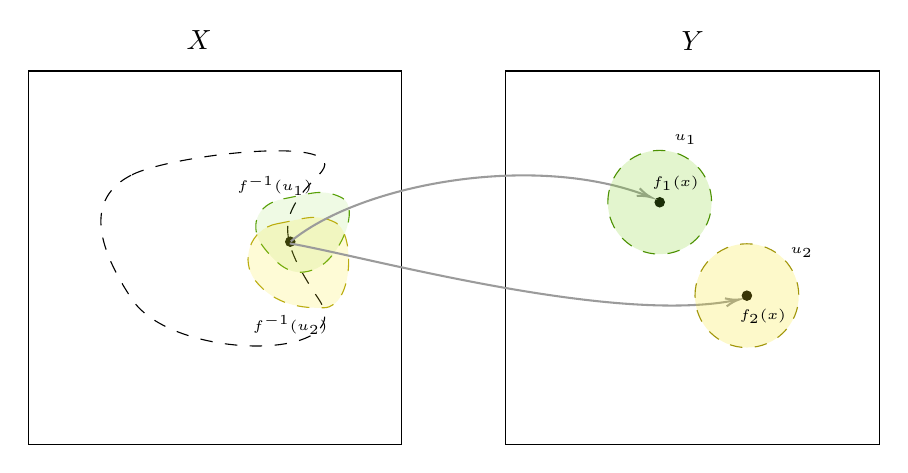
\begin{tikzpicture}[x=0.75pt,y=0.75pt,yscale=-1,xscale=1]
		%uncomment if require: \path (0,300); %set diagram left start at 0, and has height of 300
		
		%Shape: Circle [id:dp22945492936875378] 
		\draw  [fill={rgb, 255:red, 0; green, 0; blue, 0 }  ,fill opacity=1 ] (352,103.25) .. controls (352,102.01) and (353.01,101) .. (354.25,101) .. controls (355.49,101) and (356.5,102.01) .. (356.5,103.25) .. controls (356.5,104.49) and (355.49,105.5) .. (354.25,105.5) .. controls (353.01,105.5) and (352,104.49) .. (352,103.25) -- cycle ;
		%Shape: Square [id:dp934029333497959] 
		\draw   (50,40) -- (230,40) -- (230,220) -- (50,220) -- cycle ;
		%Shape: Square [id:dp16895777662650313] 
		\draw   (280,40) -- (460,40) -- (460,220) -- (280,220) -- cycle ;
		%Shape: Polygon Curved [id:ds9787457593928202] 
		\draw  [dash pattern={on 4.5pt off 4.5pt}] (100,90) .. controls (120,80) and (210,70) .. (190,90) .. controls (170,110) and (170,120) .. (190,150) .. controls (210,180) and (120,180) .. (100,150) .. controls (80,120) and (80,100) .. (100,90) -- cycle ;
		%Shape: Circle [id:dp057154404925263025] 
		\draw  [fill={rgb, 255:red, 0; green, 0; blue, 0 }  ,fill opacity=1 ] (174,122.25) .. controls (174,121.01) and (175.01,120) .. (176.25,120) .. controls (177.49,120) and (178.5,121.01) .. (178.5,122.25) .. controls (178.5,123.49) and (177.49,124.5) .. (176.25,124.5) .. controls (175.01,124.5) and (174,123.49) .. (174,122.25) -- cycle ;
		%Shape: Polygon Curved [id:ds5815057190055555] 
		\draw  [color={rgb, 255:red, 88; green, 160; blue, 7 }  ,draw opacity=1 ][fill={rgb, 255:red, 126; green, 211; blue, 33 }  ,fill opacity=0.12 ][dash pattern={on 4.5pt off 4.5pt}] (173,101.58) .. controls (186.5,99.08) and (191.5,96.42) .. (201,101) .. controls (210.5,105.58) and (200,130.08) .. (189,135.08) .. controls (178,140.08) and (171,134.58) .. (163.5,125.08) .. controls (156,115.58) and (159.5,104.08) .. (173,101.58) -- cycle ;
		%Shape: Polygon Curved [id:ds30989547801826567] 
		\draw  [color={rgb, 255:red, 187; green, 173; blue, 15 }  ,draw opacity=1 ][fill={rgb, 255:red, 248; green, 231; blue, 28 }  ,fill opacity=0.18 ][dash pattern={on 4.5pt off 4.5pt}] (170,113.58) .. controls (183.5,111.08) and (188.5,108.42) .. (198,113) .. controls (207.5,117.58) and (207,153.58) .. (192.5,154.08) .. controls (178,154.58) and (167,150.58) .. (159.5,141.08) .. controls (152,131.58) and (156.5,116.08) .. (170,113.58) -- cycle ;
		%Curve Lines [id:da29321026202366296] 
		\draw [color={rgb, 255:red, 155; green, 155; blue, 155 }  ,draw opacity=1 ][line width=0.75]    (176.5,122.08) .. controls (210.41,94.22) and (293.92,79.11) .. (348.36,100.19) ;
		\draw [shift={(350,100.84)}, rotate = 202.06] [color={rgb, 255:red, 155; green, 155; blue, 155 }  ,draw opacity=1 ][line width=0.75]    (6.56,-1.97) .. controls (4.17,-0.84) and (1.99,-0.18) .. (0,0) .. controls (1.99,0.18) and (4.17,0.84) .. (6.56,1.97)   ;
		%Curve Lines [id:da39067447551600165] 
		\draw [color={rgb, 255:red, 155; green, 155; blue, 155 }  ,draw opacity=1 ][line width=0.75]    (176,123.08) .. controls (211.15,129.02) and (330.58,162.4) .. (390.7,150.45) ;
		\draw [shift={(392.5,150.08)}, rotate = 167.68] [color={rgb, 255:red, 155; green, 155; blue, 155 }  ,draw opacity=1 ][line width=0.75]    (6.56,-1.97) .. controls (4.17,-0.84) and (1.99,-0.18) .. (0,0) .. controls (1.99,0.18) and (4.17,0.84) .. (6.56,1.97)   ;
		%Shape: Circle [id:dp16543584587564597] 
		\draw  [fill={rgb, 255:red, 0; green, 0; blue, 0 }  ,fill opacity=1 ] (394,148.25) .. controls (394,147.01) and (395.01,146) .. (396.25,146) .. controls (397.49,146) and (398.5,147.01) .. (398.5,148.25) .. controls (398.5,149.49) and (397.49,150.5) .. (396.25,150.5) .. controls (395.01,150.5) and (394,149.49) .. (394,148.25) -- cycle ;
		%Shape: Circle [id:dp376925694074147] 
		\draw  [color={rgb, 255:red, 76; green, 145; blue, 2 }  ,draw opacity=1 ][fill={rgb, 255:red, 126; green, 211; blue, 33 }  ,fill opacity=0.22 ][dash pattern={on 4.5pt off 4.5pt}] (329.25,103.25) .. controls (329.25,89.44) and (340.44,78.25) .. (354.25,78.25) .. controls (368.06,78.25) and (379.25,89.44) .. (379.25,103.25) .. controls (379.25,117.06) and (368.06,128.25) .. (354.25,128.25) .. controls (340.44,128.25) and (329.25,117.06) .. (329.25,103.25) -- cycle ;
		%Shape: Circle [id:dp3499499601701357] 
		\draw  [color={rgb, 255:red, 162; green, 150; blue, 10 }  ,draw opacity=1 ][fill={rgb, 255:red, 248; green, 231; blue, 28 }  ,fill opacity=0.23 ][dash pattern={on 4.5pt off 4.5pt}] (371.25,148.25) .. controls (371.25,134.44) and (382.44,123.25) .. (396.25,123.25) .. controls (410.06,123.25) and (421.25,134.44) .. (421.25,148.25) .. controls (421.25,162.06) and (410.06,173.25) .. (396.25,173.25) .. controls (382.44,173.25) and (371.25,162.06) .. (371.25,148.25) -- cycle ;
		
		% Text Node
		\draw (125,19.4) node [anchor=north west][inner sep=0.75pt]    {$X$};
		% Text Node
		\draw (363.5,19.9) node [anchor=north west][inner sep=0.75pt]    {$Y$};
		% Text Node
		\draw (349.5,89.4) node [anchor=north west][inner sep=0.75pt]  [font=\tiny]  {$f_{1}( x)$};
		% Text Node
		\draw (391.5,153.4) node [anchor=north west][inner sep=0.75pt]  [font=\tiny]  {$f_{2}( x)$};
		% Text Node
		\draw (360,69.4) node [anchor=north west][inner sep=0.75pt]  [font=\tiny]  {$u_{1}$};
		% Text Node
		\draw (416,123.9) node [anchor=north west][inner sep=0.75pt]  [font=\tiny]  {$u_{2}$};
		% Text Node
		\draw (149.5,89.4) node [anchor=north west][inner sep=0.75pt]  [font=\tiny]  {$f^{-1}( u_{1})$};
		% Text Node
		\draw (157,156.4) node [anchor=north west][inner sep=0.75pt]  [font=\tiny]  {$f^{-1}( u_{2})$};
		
		
	\end{tikzpicture}
\end{figure}
	
	\FloatBarrier
\end{proof}

\begin{remark}
	The theorem above indicates that if two continouse function from $\R \to \R$, agree on all values of the form $m/2^n$, for all $m\in\Z$ and $n\in \Z$, then they should agree on the whole real line.
\end{remark}

\section{Continuity and Compactness}
The compactness of the domain of a continouse function has many interesting implications.

\begin{theorem}[Continouse image of a compact set]
	Let $f:X\to Y$ be a continouse function, and $X$ compact. Then $f(X)$ is compact in $Y$.
\end{theorem}
\begin{proof}
	Let $\mathcal{G} = \{G_\alpha\}_{\alpha\in I}$ be an open cover for $f(X)$. Then we claim that $\tilde{\mathcal{G}} = \{ \inv{f}(G_\alpha) \}_{\alpha \in I}$ is also an open cover for $X$. That is because
	\[ \forall x \in X,\ \exists \alpha \in I \st f(x) \in G_\alpha \implies x \in \inv{f}(G_\alpha),\]
	thus the $\tilde{\mathcal{G}}$ covers every element of the set $X$. Since $X$ is compact, then there exists a finite sub-cover. I.e. there exists $I' \subseteq I$ finite such that $\tilde{\mathcal{G}}' = \{  \inv{f}(G_\alpha)  \}_{\alpha \in I'}$ is a finite cover for $X$. Now we claim that $\mathcal{G}' = \{  G_\alpha \}_{\alpha \in I'}$ is also a finite sub-cover for $f(X)$. This is true since for every $y \in f(X)$ we have
	\[ \inv{f}(y) \in X \implies \exists \alpha \in I' \st \inv{f}(y) \in \inv{f}(G_\alpha) \implies y \in G_\alpha. \]
	Thus $\mathcal{G}'$ covers every element of the set $f(X)$, thus it is a valid finite sub-cover for $\mathcal{G}$. This completes the proof.
\end{proof}
\newpage
\chapter{Integration}

Integrals, are one of the very central notions in the world of analysis that has numerous rules both in developing new foundational theories as well as lots of uses in the word of applications. Integrals act as a very useful norm in different spaces of functions, they help us in generalizing the notion of derivative (weak derivative), they act like linear operators between function spaces, they appear in some of the most important formulations of the natural sciences (like calculus of variations), and many many more applications. Here in this chapter we will cover the basics of the notion of integration of \emph{real} functions, and later we will see other variations of the integrals. To avoid unnecessary abstraction, we will mainly deal with functions from reals to reals, but it will be very straight forward to generalize these concepts to the complex valued functions, or function defined on $\R^n$ to $\R^m$. We start with the notion of Riemann integrable functions.

\section{Riemann Integrable Functions}
\begin{definition}[Riemann Integrable Functions]
	Let $f$ be a bounded real function define on $[a,b] \subset \R$. Let partition $P$ be the set of points $\set{x_i \in [a,b]\ :\ a=x_0 \leq x_1\leq x_2\leq x_3\leq \cdots \leq x_n=b}$ for some $n\in \N$. define $\Delta x_i = x_{i} - x_{i-1}$, and
	\[ M_i = \sup_{x\in[x_{i-1},x_{i}]}f(x), \qquad m_i = \inf_{x\in[x_{i-1},x_{i}]}f(x). \]
	Then define the following sums
	\[ U(P,f) = \sum_{i=1}^{n} M_i \Delta x_i, \qquad L(P,f) = \sum_{i=1}^{n}  m_i \Delta x_i.\]
	We define the upper and lower Riemann sums as
	\[ \overline{\int_a^b} f\ dx = \inf U(P,f), \qquad \underline{\int_a^b} f\ dx = \sup L(P,f),
	 \]
	which are called upper and lower Riemann integrals respectively. Note that the suprimum and the infimum are take on all possible partitions. \\
	We say that the function $f$ is Riemann integrable and write it as $R \in\mathcal{R}$ if 
	\[ \overline{\int_a^b} f\ dx = \underline{\int_a^b} f\ dx . \]
	And we denote this common value as
	\[ \int_a^b f\ dx. \]
\end{definition}

\begin{remark}
	Note that the upper and lower Riemann integrals exists, as in the definition we assumed that the function $f$ is bounded. If $f$ is not bounded, then $M_i$ or $m_i$ might not exist for some interval $[x_{i-1}, x_i]$, leading that the upper or lower Riemann sum might not exist. 
\end{remark}
At this point, this definition might seem useless as we are talking about things like the suprimum or infimum on all possible partitions. The set of all partitions of $[a,b]$ seems to be a set that is hard to characterize. However, as we will see, this ``hard to use'' definition will take us to somewhere that is very interesting. However, at this stage, the following example is aimed to emphasis the subtleties of the definition above.
\begin{example}[Attempting to integrate $f(x)=x$]
	Let $f: [0,1] \to \R$ where $f(x)=x$. We want to use the definition above to calculate the integral of $f(x)$ in $[0,1]$. To start with something, first, we want to consider a equidistant partition of the interval $[0,1]$ to $n$ intervals that all has the same length. Then the partition will be $P = \set{\frac{0}{n},\frac{1}{n},\cdots,\frac{n-1}{n},\frac{n}{n}}$. Then we will have
	\[ M_i = \sup_{x\in I_n} f(x) = \frac{i}{n}, \qquad m_i = \inf_{x\in I_n} f(x) = \frac{i-1}{n}, \qquad \Delta x_i = \frac{1}{n}. \]
	So the upper and lower Riemann sums will be
	\begin{align*}
		U(P,f) &= \sum_{i=1}^{n} M_i \Delta x_i = \frac{1}{n^2} \sum_{i=1}^{n}i = \frac{n(n+1)}{2n^2} = \frac{1}{2} + \frac{1}{2n^2}, \\
		L(P,f) &= \sum_{i=1}^{n} m_i \Delta x_i = \frac{1}{n^2} \sum_{i=1}^{n}(i-1) = \frac{n(n-1)}{2n^2} = \frac{1}{2} - \frac{1}{2n^2}
	\end{align*}
	Now, it is quite clear that out of all possible equidistence partitions, the infimum of $U(P,f)$ will be $1/2$, and the suprimum of $L(P,f)$ will be $1/2$ as well. \textbf{But}, I need to emphasis that this does not imply anything about the upper and lower Riemann integrals. That is because, the upper (lower) Riemann sum is the infimum (suprimum) considered on all partitions. However, here, we have only considered the partitions with equal distance intervals. However, one might come up with an elegantly designed partition that can change the game. This at this stage, we can not even integrate the function $f(x) = x$. We will make our original definition of Riemann integrablity by a very useful generalization to the Riemann-Stieltjes integrals.
\end{example}

\begin{proposition}[Properties of the Riemann sums]
	Let $f: [a,b] \to \R$ bounded, and let $P$ be any partition. Then we have
	\begin{enumerate}[(a)]
		\item $L(P,f) \leq U(P,f).$
		\item $\exists m,M \in \R$ such that $m(b-a) \leq L(P,f) \leq U(P,f) \leq M(b-a)$.
	\end{enumerate}

\end{proposition}
\begin{proof}
	\begin{enumerate}[(a)]
		\item This follows immediately from the properties of suprimum and infimum.
		\item Since $f$ is bounded, then $\exists m,M \in \R$ such that $m \leq f(x) \leq M\ \forall x \in [a,b]$. Then
		\begin{align*}
			U(P,f) &= \sum_{i=1}^{n} M_i \Delta x_i \leq \sum_{i=1}^{n} M \Delta x_i = M \sum_{i=1}^{n} \Delta x_i  = M(b-a),\\
			L(P,f) &= \sum_{i=1}^{n} m_i \Delta x_i \geq \sum_{i=1}^{n} m \Delta x_i = m \sum_{i=1}^{n} \Delta x_i  = m(b-a).
		\end{align*}
		Note that we use the telescoping property of the sums above. Combining the results from above with the result of part (a) we can write
		\[ m(b-a) \leq L(P,f) \leq U(P,f) \leq M(b-a). \] 
	\end{enumerate}
\end{proof}

\section{Riemann-Stieltjes Integrals}
At this point we will generalize the notion of Riemann integration to Riemann-Stieltjes integration. The idea behind this generalization will be more clear later. 

\begin{definition}[Riemann-Stieltjes Integrals]
	TO BE ADDED
\end{definition}

The following definition of the refinement of a partition, will help up to prove some statements that will help us in making useful tools out of the definitions above.
\begin{definition}[Refinement of a partition]
	We say that the partition $P^*$ is a refinement of the partition $P$ if $P \subseteq P^*$. Given two partitions $P_1, P_2$, their \textbf{common refinement} is the partition $P = P_1 \cup P_2$.
\end{definition}
The following theorem will show the significance of the notion of the refinements.
\begin{lemma}
	If $P^*$ is a refinement of $P$, then we have
	\begin{enumerate}[(i)]
		\item $L(P,f,\alpha) \leq L(P^*,f,\alpha)$
		\item $U(P^*,f,\alpha) \leq L(P, f, \alpha)$
	\end{enumerate}
\end{lemma}
\begin{proof}
	We will prove the first statement, and the proof for the second statement will be analogous. First, assume that the refinement $P^*$ has only one extra point, say $x^*$ that falls in the $i$-th interval i.e. $I_i = [x_{i-1}, x_i]$. Thus this interval will turn into two intervals $I_i^{(1)} = [ x_{i-1}, x^* ]$ and $I_i^{(2)} = [x^*, x_i]$. Let 
	\[ M_i = \sup_{x\in I_i f(x)}f(x),\qquad w_1 = \sup_{x\in I_i^{(1)}}f(x),\qquad w_2 = \sup_{x\in I_i^{(2)}}f(x). \]
	Then, from the properties of suprimum it follows that $w_2 \leq M_i$ and also $w_1 \leq M_i$. Then 
	\[ U(P,f,\alpha) - U(P^*,f,\alpha) = M_i(\alpha_{i} - \alpha_{i-1}) - \left( w_1(\alpha(x^*) - \alpha_{i-1}) + w_2(\alpha_i - \alpha(x^*)) \right) \]
	Since $w_1 \leq M_i$, and $w_2 \leq M_i$, and $\alpha$ is non-decreasing, then
	\[ w_1 (\alpha(x^*) - \alpha_{i-1}) \leq M_i(\alpha(x^*) - \alpha_{i-1}),\quad w_2 (\alpha(x^*) - \alpha_{i-1}) \leq M_i(\alpha(x^*) - \alpha_{i-1}) \]
	Then we can write
	\[ U(P,f,\alpha) - U(P^*,f,\alpha) \geq M_i(\alpha_i - \alpha_{i-1}) - M_i(\alpha_i - \alpha_{i-1}) = 0. \]
	then it immediately follows that
	\[ U(P^*,f,\alpha) \leq U(P,f,\alpha) \]
\end{proof}

The following important proposition will take advantage of the lemma above.

\begin{proposition}
	Let $f:[a,b] \to \R$ bounded, and $\alpha:[a,b] \to \R$ non-decreasing.
	Then 
	\[ \underline{\int_a^b} f\ d\alpha \leq \overline{\int_a^b} f\ d\alpha. \]
		\label{thm:LowerIntLessThanUpperIng_RS}
\end{proposition}
\begin{proof}
%	We will not be very concise in the steps of this proof, as we want to also demonstrate the line of thought in processing such theorems. Let $\tilde{P}$ be the set of all partitions of $[a,b]$. Then
%	\[ \tilde{U} = \set{U(P,f,\alpha)\ :\ P \in \tilde{P}}, \qquad \tilde{L} = \set{L(P,f,\alpha)\ :\ P \in \tilde{P}}. \]
%	$\tilde{U}$ and $\tilde{L}$ are subsets of real numbers. Then it is clear that 
%	\[  \underline{\int_a^b} f\ d\alpha = \sup \tilde{L}, \qquad \overline{\int_a^b} f\ d\alpha = \inf \tilde{U}. \]
%	Let $A = \sup \tilde{L}$, and $B = \sup\tilde{U}$. With the new terminology, we need to prove $A \leq B$.\\
%	We will proceed with the proof by contradiction. Assume $B < A$. Since $A$ is the suprimum of $\tilde{L}$, then $B<A$ implies there exists a partition $P_1 \in \tilde{P}$ such that 
%	\[ B < L(P_1, f, \alpha) \leq A. \]
%	Similarly, we can find $P_2 \in \tilde{P}$ such that 
%	\[ B \leq U(P_2, f, \alpha) < A. \]
	
	Let set $\mathbb{P}$ denote the set of all partitions on the interval $[a,b]$. Then for $P_1, P_2 \in \mathbb{P}$, let their common refinement be $P^* = P_1 \cup P_2$. Then from the properties of the common refinement we can write
	\[  L(P_1,f,\alpha) \leq L(P^*,f, \alpha), \qquad U(P^*, f,\alpha) \leq U(P_1, f, \alpha). \]
	However, it follows from the properties of the upper and lower Riemann sums for partition $P^*$ that
	\[ L(P^*,f,\alpha) \leq U(P^*,f,\alpha). \]
	Combining these two results will lead to 
	\[ L(P_1,f,\alpha) \leq L(P^*,f,\alpha)\leq U(P^*,f,\alpha) \leq U(P_2,f,\alpha) \qquad \forall P_1,P_2 \in \mathcal{P} \]
	If $P_2$ is fixed, then taking $\sup$ on all $P_1 \in \mathcal{P}$ we will have
	\[ \underline{\int_{a}^{b}}f\ d\alpha \leq U(P_2,f,\alpha).\]
	Now by taking $\inf$ on all $P_2 \in \mathcal{P}$ we will have
	\[ \underline{\int_{a}^{b}}f\ d\alpha \leq \overline{\int_{a}^{b}}f\ d\alpha. \]
\end{proof}
The following theorem comes very handy in the applications.
\begin{theorem}
	$f \in \mathcal{R}_\alpha[a,b]$ if and only if $\forall \epsilon>0$ there exists a partition such that 
	\[ U(P,f,f\alpha) - L(P,f,\alpha) < \epsilon. \]
\end{theorem}
\begin{proof}$\ $ \\
	\noindent $\boxed{\Longrightarrow}$ We assume $f\in \mathcal{R}_\alpha[a,b]$. Then 
	\[ \underline{\int_{a}^{b}}f\ d\alpha = \overline{\int_{a}^{b}}f\ d\alpha = I \]
	Since $I = \inf_{p\in\mathcal{P}}U(P,f,\alpha)$, then there exists $P_1 \in\mathcal{P}$ such that 
	\[ U(P_1,f,\alpha) < I + \epsilon/2. \]
	Similarly, $\exists P_2 \in \mathcal{P_2}$ such that
	\[ L(P_2,f,\alpha) > I - \epsilon/2. \]
	Let $P^*$ be the common refinement of $P_1, P_2$. I.e. $P^* = P_1\cup P_2$. Then 
	\[ I-\epsilon/2 < L(P_2,f,\alpha)\leq L(P^*,f,\alpha)\leq U(P^*,f,\alpha) \leq U(P_1,f,\alpha) < I + \epsilon/2. \]
	Then the maximum difference between $U(P^*,f,\alpha)$ and $L(P^*,f,\alpha)$ can be $\epsilon$. I.e.
	\[ U(P^*,f,\alpha) - L(P^*,f,\alpha) < \epsilon. \]
	\noindent $\boxed{\Longleftarrow}$ We can do this in two different ways. For the first method, I will use the proof by contradiction. But to do this, first observe that $\inf_{P \in \mathbb{P}} U(P,f,\alpha)$ and $\sup_{P\in \mathbb{P}}L(U,f,\alpha)$ exists. That is because if $\inf_{P \in \mathbb{P}}U(P,f,\alpha) = -\infty$, then $\sup_{P\in \mathbb{P}}L(P,f,\alpha) = -\infty$ as well. Similarly, if $\sup_{P\in \mathbb{P}}L(P,f,\alpha)=\infty$, then $\inf_{P \in \mathbb{P}}L(P,f,\alpha) = \infty$ as well. In either case, the hypothesis fails to be true. Thus $\exists \gamma_1, \gamma_2 \in \R$ such that $\gamma_1 = \inf_{P \in \mathbb{P}}U(P,f,\alpha)$ and $\gamma_2 = \sup_{P\in \mathbb{P}}L(P,f,\alpha)$. From \autoref{thm:LowerIntLessThanUpperIng_RS} it follows that $\gamma_2 \leq \gamma_1$. We claim that $\gamma_2 = \gamma_1$. Because other wise, we let $\epsilon = \gamma_1 - \gamma_2$. Then by hypothesis we can find $P \in \mathbb{P}$ such that 
	\[ U(P,f,\alpha) - L(P,f,\alpha) < \epsilon. \] On the other hand, from the properties of sup and inf we know that
	\[ U(P,f,\alpha) \geq \gamma_1, \qquad L(P,f,\alpha) \leq \gamma_2\]
	Thus it follows 
	\[ U(P,f,\alpha) - L(P,f,\alpha) \geq \epsilon,\]
	which is a contradiction.\\
	There is also a much more higher level proof that utilizes the previous results. Let $\epsilon>0$ given. Then $\exists P \in \mathbb{P}$ such that
	\[ U(P,f,\alpha) - L(P,f,\alpha) < \epsilon. \]
	We know that for all $P \in \mathbb{P}$ we have
	\[ L(P,f,\alpha) \leq \underline{\int}f\ d\alpha \leq \overline{\int}f\ d\alpha  \leq U(P,f,\alpha). \]
	Thus
	\[ 0 \leq \overline{\int}f\ d\alpha - \underline{\int}f\ d\alpha  < \epsilon. \]
	However, since this is true for any $\epsilon>0$, then we can conclude that the upper and lower integrals are equal, thus $f \in \mathcal{R}_\alpha[a,b]$.
\end{proof}
\begin{corollary}
	Let $f:[a,b]\to\R$ be bounded. Assume for some $\epsilon>0$ and some partition $P \in \mathcal{P}$ we have
	\[ U(P,f,\alpha) - L(P,f,\alpha) < \epsilon. \]
	Then this holds for every refinement of $P$ (With the same $\epsilon$).
\end{corollary}
\begin{proof}
	Let $P^*$ be any refinement of $P$. Then 
	\[ L(P,f,\alpha) \leq L(P^*,f,\alpha),\qquad U(P^*,f,\alpha)\leq U(P,f,\alpha).  \]
	We can rearrange this as
	\[ L(P,f,\alpha) \leq L(P^*,f,\alpha) \leq U(P^*,f,\alpha) \leq U(P,f,\alpha). \]
	The it immediately follows that
	\[ U(P^*,f,\alpha) - L(P^*,f,\alpha) < \epsilon. \]
\end{proof}

The following theorem is one of our major results so far. Thus theorem highlights the fact that how we can arrive at useful results from abstract definitions. 

\begin{theorem}[Continuous functions are Riemann-Stieltjes integrable.]
	Let $f:[a,b] \to \R$ be a continuous function. Then it is Riemann-Stieltjes integrable.
\end{theorem}
\begin{proof}
	Choose $\eta$ small enough such that 
	$$(\alpha(b) - \alpha(a))\eta < \epsilon.$$
	Then since the function $f$ is continuous on a compact set $[a,b]$, it is uniformally continuous. So for $\eta$ chosen as above, we can find $\delta>0$ such that for every $t,s \in [a,b]$ we have
	\[ \abs{t-s} < \delta \implies \abs{f(t) - f(s)} < \eta. \]
	Then if $P$ is a partition that $\Delta x_i < \delta$ for all $i$, then we have
	\[ M_i - m_i < \eta. \]
	Now consider the following difference between the upper and lower Riemann sums 
	\[ U(P,f,\alpha) - L(P,f,\alpha) = \sum_{i=1}^{n} (M_i-m_i) \Delta \alpha_i \leq \sum_{i=1}^{n}\eta \Delta\alpha_i = \eta (\alpha(b) - \alpha(a)) < \epsilon.  \]
	So the function $f$ is Riemann-Stieltjes integrable.
\end{proof}

The following theorem is also useful as it relaxes some of the requirements on the function $f$ to be Riemann-Stieltjes integrable, and puts more constraints on the integrator $\alpha$. The proof will be very similar to the proof above.

\begin{theorem}
	Let $f:[a,b] \to \R$ monotone function, and $\alpha$ continuous on $[a,b]$. Then $f \in \mathcal{R}_\alpha[a,b]$ (note that we still require $\alpha$ to be monotone). 
\end{theorem}
\begin{proof}
	Assume that the function $f$ is non-decreasing (the proof for the other case will be analogous). For a given $\epsilon>0$, choose $\eta>0$ small enough that
	\[ (f(b) - f(a))\eta < \epsilon. \]
	Since $\alpha$ is continuous on the compact set $[a,b]$, then it is uniformally continuous. Thus for chosen $\eta$ as above, we can find $\delta>0$ such that for all $t,s \in [a,b]$ we have
	\[ \abs{t-s} < \delta \implies \abs{\alpha(t) - \alpha(s)} < \eta. \]
	Let $P$ be any partition that $\Delta x_i < \delta$ for all $i$. Then $\Delta \alpha_i < \eta$ for all $i$. So we can write
	\[ \sum_{i=1}^{n} (M_i - m_i)\Delta\alpha_i < \eta \sum_{i=1}^{n} (M_i - m_i). \]
	Since $f$ is non-decreasing, then for all $i$ we have $M_i = f(x_i)$ and $m_i = f(x_{i-1})$. Then the sum above telescopes and we will have
	\[ U(P,f,\alpha) - L(P,f,\alpha) < \eta (f(b) - f(a)) < \epsilon. \]
\end{proof}

\chapter{Sequences and Series of Functions}

In this chapter we will study the sequence and series of functions. We will study different notions of convergence, namely point-wise convergence, uniform convergence, etc. Note that in this chapter, we will try to be as concrete as possible, avoiding unnecessary abstraction.

\begin{definition}[Point-wise convergence]
	Let $\seq{f}$ be a sequence of functions $f: [0,1] \to \R$. Then we say that this sequence converges \emph{point-wise} to the function $f[0,1]\to\R$, and show it as $f_n(x)\to f$ if
	\[ \forall \epsilon>0, x\in [0,1],\ \exists N>0 \st \forall n>N \wh \abs{f_n(x) - f(x)} < \epsilon.  \]
	We write this as $\lim_{n\to\infty}f_n(x) = f(x)$.
\end{definition}
\begin{remark}
	Note the order of the quantifiers in the definition above. What we are basically saying is that for any choice of $\epsilon$ and for any $x$, we can find $N$ (that depends on $\epsilon$ and $x$) such that for all $n>N$ we have $\abs{f_n(x)-f(x)}<\epsilon$. There is \textbf{NO} guarantee that by using this $N$, for any other point $x'$ we have $\abs{f_n(x') - f(x)} < \epsilon$.
\end{remark}

Thinking more carefully, we can see that this is nothing other than a collection of sequences in $\R$ that are indexed by index the set $[0,1]$. For instance, for $x=0.5$, $\set{f_n(0.5)}_n$ is a sequence in $\R$ like any other value of $x\in [0,1]$. That is why a sequence of functions can be thought of as an indexed sequence. And the point-wise notion of convergence to $f(x)$ is nothing other than indexing the converged value by $x$. Back to the previous example, for $x=0.5$, if we know that $\set{f_n(0.5)}_n$ convergence, the symbol $f(0.5)$ is the most appropriate symbol to represent the limit. Then for $x=0.6$, if $\seq{f_n(x)}$ converges, we can say it converges to $f(0.6)$. So the point-wise convergence is simply saying that all of the indexed sequences converge to a set whose values are indexed by the same index as the index of the corresponding sequence. 

Because of our discussion above, it is not surprising if we say that there is no guarantee that some good properties of $f_n$ carries over to $f$ (like continuity, differentiability, integrability, etc). That is because the point-wise notion of convergence is only expressing the convergence of a bunch of sequences (indexed with real numbers in [0,1]) in a neat way.

As we will discover through this chapter, it turns out that the question about if the properties of the function $f_n$ carries over the properties of the $f$ through the point-wise convergence, is essentially the same type of question that if in a multivariate limit, exchange of limit order is allowed. 


\begin{definition}[Uniform convergence]
	let $\set{f_n}$ be a sequence of functions $f:[0,1] \to \R$. Then we say that the sequence converges to $f: [0,1] \to \R$ if 
	\[ \forall \epsilon>0,\ \exists N>0 \st \forall n>N \wh \qquad \abs{f_n(x)-f(x)} < \epsilon \quad \forall x\in [0,1]. \]
	We show this by $f_n \to f$.
\end{definition}
\begin{remark}
	Note the order of the quantifiers and compare that closely with the definition of the point-wise convergence. In the uniform convergence, for any choice of $\epsilon$, we can find $N$ that for all $n>N$ we have $\abs{f_n(x)- f(x)} <\epsilon$ that holds true for any $x\in [0,1]$. Thus in some sense, the function $f_n$ converges to $f$ as a whole, and not in a point by point sense. This is also evident in the notation that we use to demonstrate the uniform convergence $f_n \to f$, that gives the feeling that the functions $f_n$ converges to $f$ as a whole object.
\end{remark}

\begin{theorem}[Cauchy criteria of convergence]
	Let $\set{f_n}_n$ be a sequence of functions $f_n: E \to \R$. This sequence converges to $f$ uniformally, if and only if $\forall \epsilon>0,\ \exists N>0 \st \forall n,m>N \wh \abs{f_n(x) - f_m(x)} < \epsilon \ \forall x\in E$.
\end{theorem}
\begin{proof}
	$\boxed{\implies}$ For this direction, we need to show that uniform convergence imply the sequence to be Cauchy. Let $\epsilon>0$ given. Then since $f_n \to f$, then we can find integer $N$ such that for all $n,m>N$ and $x\in E$
	\[ \abs{f_n(x)-f(x)}<\epsilon/2, \qquad \abs{f_m(x)-f(x)}<\epsilon/2 \]
	Thus we can write
	\[ \abs{f_n(x) - f_m(x)} \leq \abs{f_n(x)-f(x)} + \abs{f_m(x)+f(x)} < \epsilon \]
	
	\noindent $\boxed{\Longleftarrow}$ For this direction, we need to prove that the Cauchy criteria satisfied implies the uniform convergence. First, observe that for any fixed $x$, the sequence $\set{f_n(x)}$ is Cauchy in $\R$. Thus it converges to some real number $f(x)$. Given $\epsilon>0$ choose $N$ large enough that $\forall n,m > N$ we get
	\[ \abs{f_n(x) - f_m(x)}  < \epsilon/2 \qquad \forall x\in E.\]
	Then, for all $x\in E$ we can write
	\[ \abs{f_n(x) - f(x)} \leq \abs{f_n(x) - f_m(x)} + \abs{f_m(x) - f(x)}. \]
	The first term in the right hand side is less than $\epsilon/2$. And since $f_m(x) \to f(x)$, we can choose $m$ large enough that $\abs{f_m(x) - f(x)} < \epsilon/2$. Thus we will get
	\[ \abs{f_n(x) - f(x)} < \epsilon. \]
	This completes our proof. 
\end{proof}
\chapter{Useful Tips, Tools, and Tricks for $\R$eal Analysis}


In this chapter we will cover some useful tips and tricks in solving the problem. This is not a complete and comprehensive list of tricks, and the list will grow larger as I encounter more of these in different resources.

\begin{trick}
	There is a way to produce multiplication from squaring and addition/difference. Suppose that a set $S$ is closed under squaring, as well as addition and subtraction. Thus if $a,b \in S$ then $a+b \in S$, $a-b\in S$, thus $(a-b)^2 \in s$ as well as $(a+b)^2\in S$. Thus $(a+b)^2 - (a-b)^2 \in S$ as well. Thus
	\[  (a+b)^2 - (a-b)^2 = 4ab \in S. \]
	Thus we can conclude that being closed under addition, subtraction, and squaring, leads to being closed under multiplication as well.
\end{trick}
One useful use of this trick is in when we try to prove if $f$ and $g$ are Riemann–Stieltjes integrable, then we want prove that $fg$ is also Riemann–Stieltjes integrable. We do so by observing that $f,g$ are RS integrable, then so is $f+g$ and $f-g$ (which are proved by simpler theorem) and also $f^2$ is RS integrable. Thus from the trick above we can conclude that $fg$ is also RS integrable. 













\section{Construction Zone}
Some tricks for real analysis. I will expand this list and also explain each one with its particular use case throughout this chapter


\begin{enumerate}

\item archimedes
\item well ordering principle
\item unpack defn
\item IVT
\item MVT
\item three equiv. defn for cts.
\item sequential compactness
\item heine borel
\item bolzano weierstrass
\item lim $x_n=L$ iff limsup $x_n=\liminf x_n=L$
\item sequential characterization of open, closed sets, and others
\item union of countable set is countable
\item add subtrace and multiply divide
\item define new set or function and play with it
\item construct sequence
\item triangle inequality
\item X compact then f:X->R has max/min in X and f(X) compact
\item work backwards and apply previous results
\item contrapositives
\item denseness of Q in R
\item finite intersection prop
\item cantor intersection thm
\item squeeze thm
\item limit laws
\item monotone convergence thm
\item show seq cauchy (by completeness)
\item diff between squares
\item exploit the defn of convergence
\item consider all cases
\item maybe try proof by contradiction
\item ep ball defn of x in cl(A)
\item if A is subset of B and B closed then cl(A) is subset of B
\item if A is subset of B and A open then A subset of int(A)
\item HTS1-HTS4

\end{enumerate}




\end{document}